\chapter{HLASM overview}

In general, high-level assemblers provide for their assembly languages features that are commonly found in high-level programming languages. Hence, in addition to ordinary machine instructions they also contain control statements similar to \textit{if, while, for} as well as custom callable macros.

IBM High Level Assembler (HLASM) comforts this definition and adds other features which will be described in this chapter.

\section{Syntax}

HLASM has somehow complicated syntax.

\subsection{Statement}

HLASM program is sequence of \textit{statements}. Statement consists of four fields. Those are:
\begin{itemize}
	\item \textbf{Name field} --- Serves as place for named constants that are to be used in code.
	
	\item \textbf{Operation field} --- Instruction that is executed.
	
	\item \textbf{Operands field} --- Field for instruction operands separated by comma.
	
	\item \textbf{Remark field} --- Serves as line commentary.
\end{itemize}

\begin{verbatim}
 label   instruction     operands             remarks
.NOMOV       AGO     (&WH).L1,.L2,.L3     SEQUENTIAL BRANCH
\end{verbatim}

\subsection{Continuation}

One line in HLASM source code can contain only up to 80 characters. However, sometimes statement is too long to be written in one line. Therefore, special handling is introduced called \textbf{continuation}.

For indication that statement continues on the next line a character other than space is placed in \textbf{continuation column} (default is 72). Then the remainder of the statement must start on \textbf{continue column} (default is 15) to finally create a well formed statement (see \cref{fig01:line}).

\begin{figure}\centering
	%the extra width spec prevents overflow
	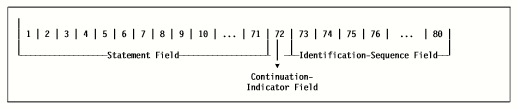
\includegraphics[width=\linewidth]{img/line}
	\caption{Description of line columns.}
	\label{fig01:line}
\end{figure}


\section{Semantics}

\subsection{Conditional assembly}

\subsection{Ordinary assembly}
